% Capitulo IV: Resultados esperados (maximo 5 paginas)

\chapter{RESULTADOS ESPERADOS}

Este capítulo expone el desempeño esperado de la sombra digital a partir de la simulación descrita en el Capítulo III. Su propósito no es validar una teoría, sino mostrar que la solución diseñada es funcional, segura y coherente con el problema planteado. La Figura~\ref{fig:concepto} resume cómo se espera que opere una vez implementada: el gateway lee el controlador del compresor por Ethernet, la sombra digital evalúa su condición y el personal de mantenimiento recibe el índice de salud, la causa probable y la acción recomendada.

\begin{figure}[htbp]
\centering
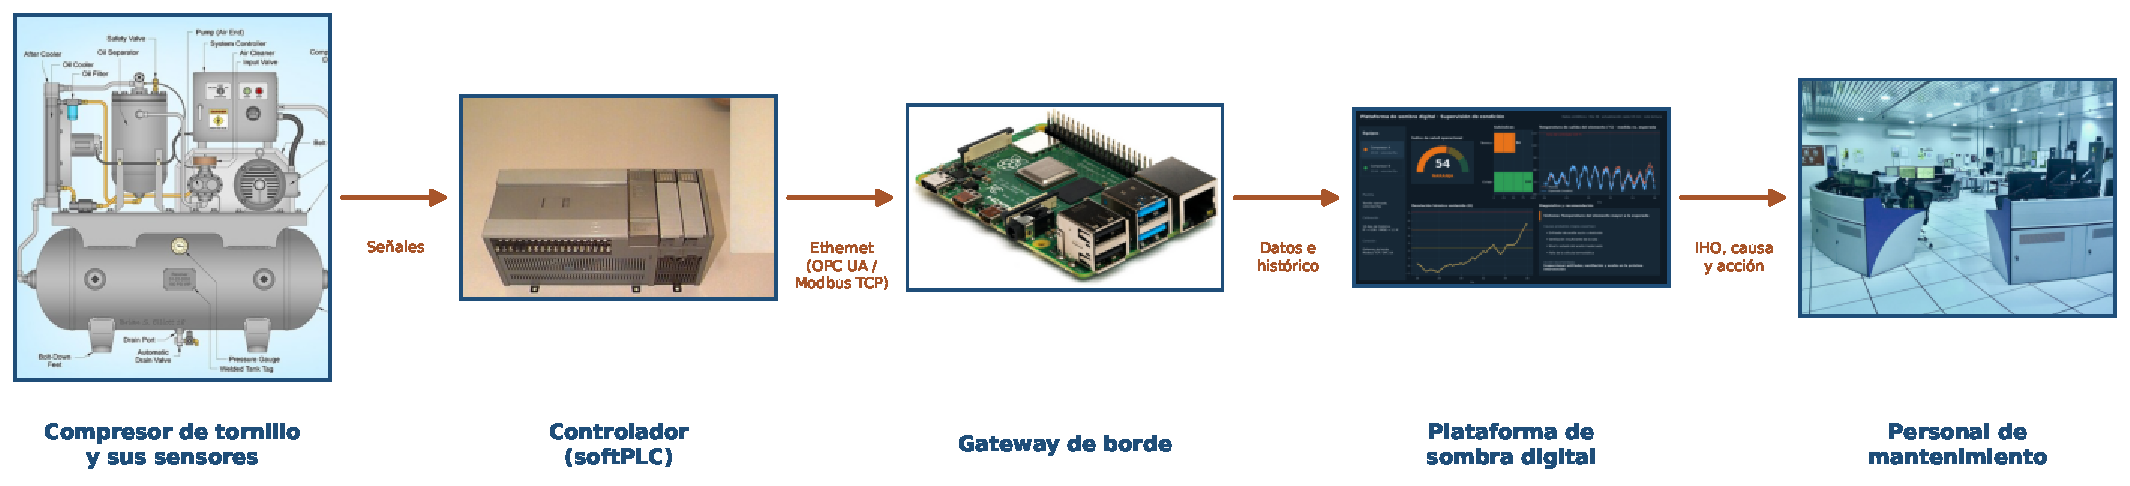
\includegraphics[width=\textwidth]{fig_concepto_implementacion.pdf}
\caption{Concepto de implementación esperado de la sombra digital. Imágenes: B. S. Elliott (CC BY-SA 4.0), Wikimedia Commons (CC BY-SA 3.0), Laserlicht (CC BY-SA 4.0) y Z22 (CC BY-SA 4.0), vía Wikimedia Commons; tablero: elaboración propia}
\label{fig:concepto}
\end{figure}

\section{Solución funcional}

Con el mismo código y cambiando solo el archivo de configuración, la sombra digital calibró un modelo distinto para cada compresor con 14 días de histórico y detectó los dos escenarios de degradación en ambos equipos (Tabla~\ref{tab:desempeno}). En el compresor A, la alerta amarilla del escenario térmico se confirmó 3 días después del inicio de la falla y unos 23 días antes del aviso por alta temperatura del controlador, ya que la temperatura todavía estaba por debajo de 110\,°C, pero era mayor que la esperada para las condiciones de operación (Figura~\ref{fig:termico}). El ciclaje excesivo, que el controlador no advierte, se detectó entre 5 y 11 días después de iniciado.

\begin{table}[htbp]
\centering
\caption{Desempeño esperado de la sombra digital en dos equipos (10 simulaciones por escenario)}
\label{tab:desempeno}
\footnotesize
\renewcommand{\arraystretch}{1.3}
\begin{tabular}{|p{7.0cm}|p{3.0cm}|p{3.0cm}|}
\hline
\textbf{Indicador} & \textbf{Compresor A} & \textbf{Compresor B} \\ \hline
Potencia y temperatura media de la sala (supuestas) & 45\,kW; 24\,°C & 22\,kW; 28\,°C \\ \hline
$R^2$ y RMSE del modelo calibrado & 0,962; 1,13\,K & 0,965; 1,45\,K \\ \hline
Térmico: días hasta el nivel amarillo & 3,2 $\pm$ 0,7 & 3,1 $\pm$ 0,5 \\ \hline
Térmico: anticipación frente al aviso del controlador & 23,5 $\pm$ 1,8 días & 16,0 $\pm$ 2,2 días \\ \hline
Ciclaje: días hasta el nivel amarillo & 11,2 $\pm$ 2,2 & 4,8 $\pm$ 1,2 \\ \hline
Tiempo fuera de verde sin falla & 0,00\,\% & 0,33\,\% \\ \hline
\end{tabular}
\end{table}

\begin{figure}[htbp]
\centering
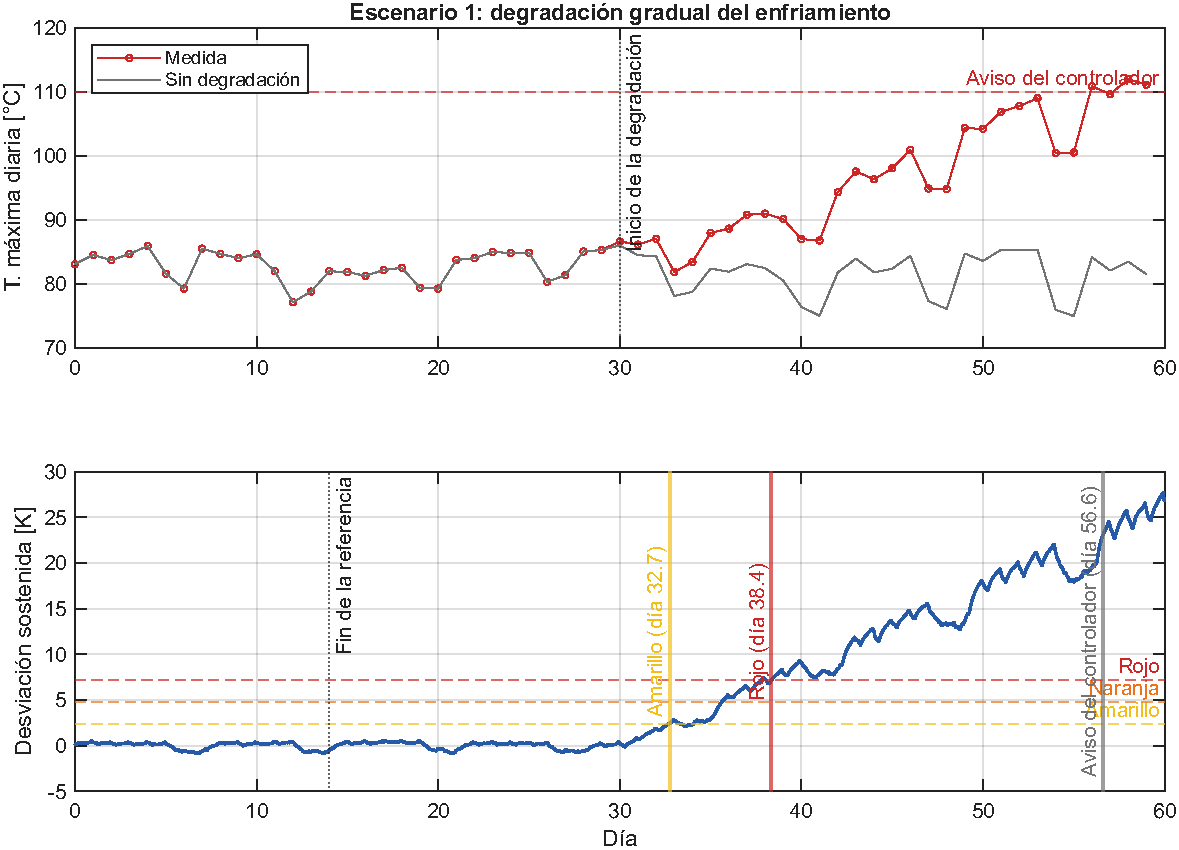
\includegraphics[width=0.9\textwidth]{fig_escenario_termico.pdf}
\caption{Escenario térmico del compresor A: temperatura máxima diaria y desviación sostenida}
\label{fig:termico}
\end{figure}

La Figura~\ref{fig:plataforma} muestra el índice de salud operacional de ambos equipos. En operación normal se mantuvo en verde, y en los escenarios de falla descendió de forma progresiva por los cuatro niveles. En cada caso, la base de reglas identificó el síntoma correcto y emitió la acción recomendada: inspeccionar el enfriador, la ventilación y el aceite ante la anomalía térmica, y revisar el purgador y la banda de presión ante el ciclaje.

\begin{figure}[htbp]
\centering
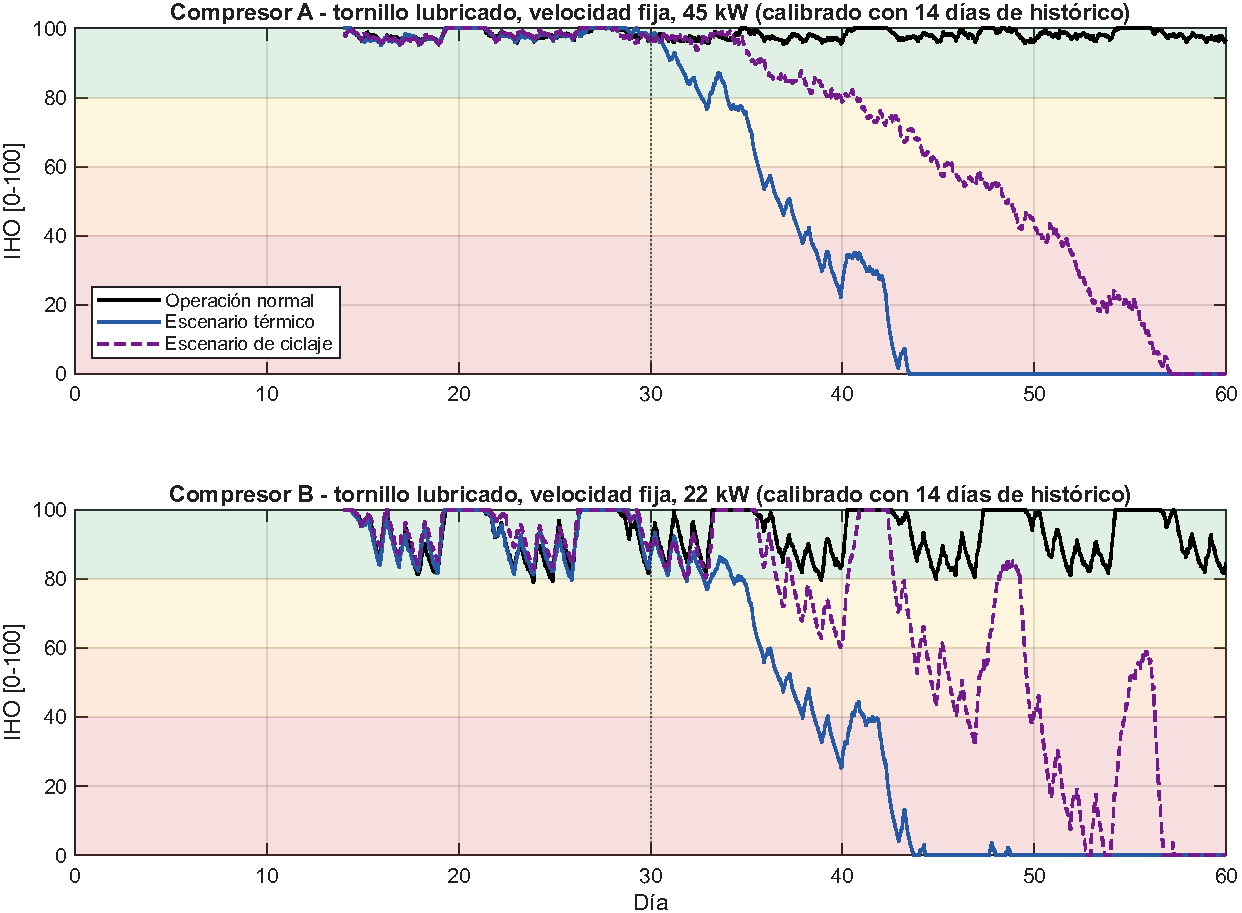
\includegraphics[width=0.9\textwidth]{fig_plataforma_iho.pdf}
\caption{Índice de salud operacional de los dos equipos calibrados por la sombra digital}
\label{fig:plataforma}
\end{figure}

La Figura~\ref{fig:tablero} muestra la vista esperada del tablero para el compresor A en el día 36 del escenario térmico: el índice en nivel naranja, la temperatura medida por encima de la esperada aunque lejos del aviso del controlador, la desviación sostenida frente a los umbrales y el diagnóstico con sus causas probables y la acción recomendada.

\begin{figure}[htbp]
\centering
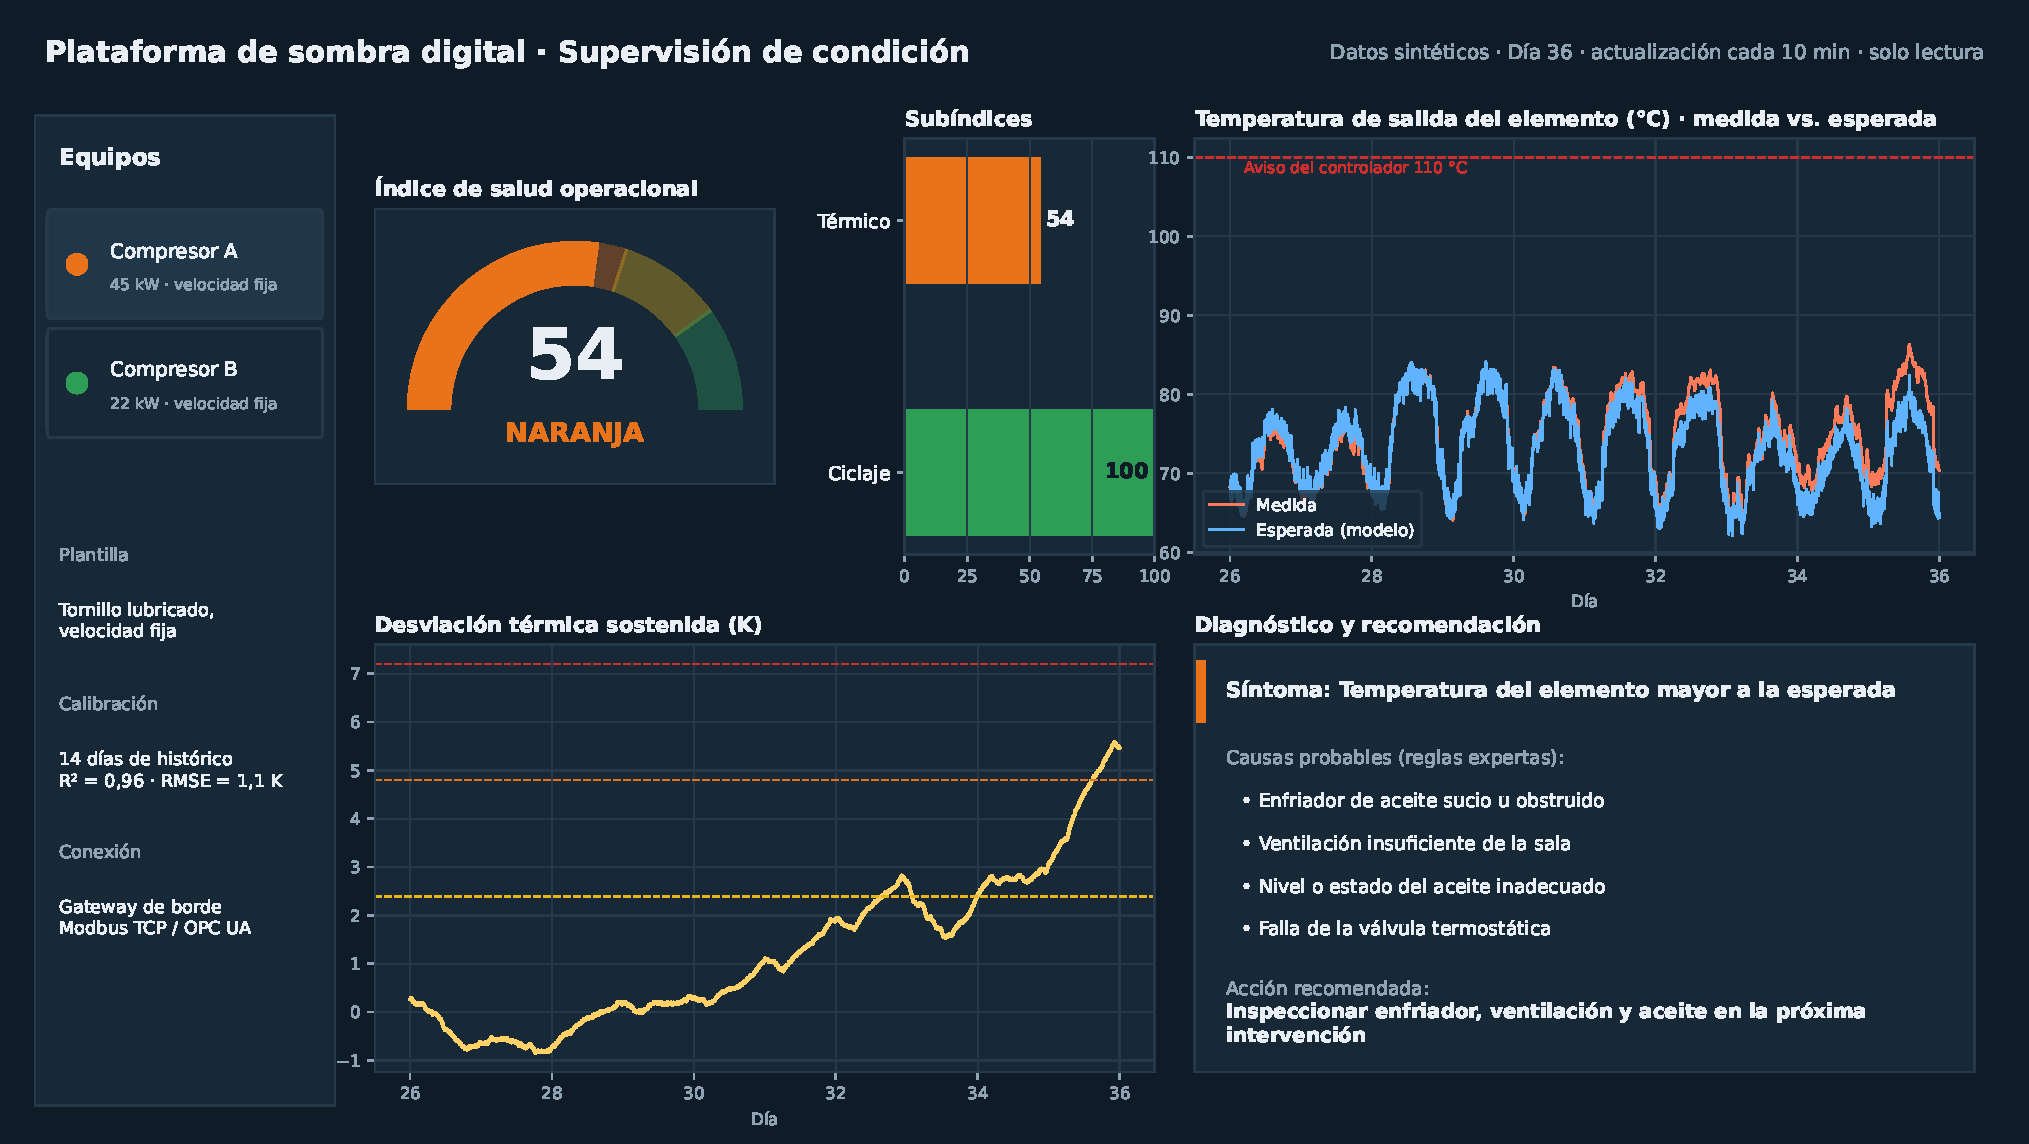
\includegraphics[width=\textwidth]{fig_tablero.pdf}
\caption{Vista esperada del tablero de la sombra digital (elaboración propia con datos sintéticos)}
\label{fig:tablero}
\end{figure}

\section{Solución segura}

La sombra digital solo lee los datos del controlador y entrega recomendaciones al personal; no modifica consignas ni protecciones, por lo que las alarmas y paradas del equipo se mantienen intactas. Respecto a la confiabilidad de las alertas, el tiempo fuera de verde sin falla fue menor al 1\,\% en ambos equipos. Para estimar el efecto de condiciones no representadas en el modelo, como la humedad o un sensor descalibrado, se agregó a la temperatura del compresor A una perturbación lenta: con 1\,K no hubo alertas sin causa, con 2\,K el índice salió de verde el 3,8\,\% del tiempo y con 3\,K, el 12,4\,\%, sin dejar de detectar la falla. En consecuencia, en una implementación real los umbrales deberán calibrarse con datos del equipo.

\section{Solución coherente con el problema}

La Tabla~\ref{tab:cumplimiento} contrasta los resultados con los requerimientos derivados del problema.

\begin{table}[htbp]
\centering
\caption{Cumplimiento de requerimientos}
\label{tab:cumplimiento}
\footnotesize
\renewcommand{\arraystretch}{1.3}
\begin{tabular}{|p{0.7cm}|p{4.6cm}|p{5.6cm}|p{2.0cm}|}
\hline
\textbf{ID} & \textbf{Criterio} & \textbf{Resultado esperado} & \textbf{Estado} \\ \hline
R1 & Anticipación mínima de 7 días & 23,5 días (A) y 16,0 días (B) & Cumple \\ \hline
R2 & Alerta ante un aumento de ciclos de 20\,\% & Nivel amarillo al superar el 20\,\% & Cumple \\ \hline
R3 & Menos del 5\,\% fuera de verde sin falla & 0,00\,\% (A), 0,33\,\% (B); 3,8\,\% con 2\,K & Cumple \\ \hline
R4 & Acceso de solo lectura & Sin órdenes al controlador & Por diseño \\ \hline
R5 & Índice, causa probable y acción & IHO con semáforo y reglas expertas & Cumple \\ \hline
R6 & Sin sensores adicionales & Solo variables del controlador & Por diseño \\ \hline
R7 & Calibración con 14 días de datos & Un modelo por equipo & Cumple \\ \hline
R8 & RMSE de validación menor a 2\,K & 1,13\,K (A) y 1,45\,K (B) & Cumple \\ \hline
\end{tabular}
\end{table}

Los resultados son esperados con datos sintéticos y parámetros de diseño; su validación con datos reales del compresor queda como etapa posterior a este proyecto.
